\documentclass{beamer}

\usepackage[italian]{babel}
\usepackage[utf8]{inputenc}
\usepackage{graphicx}

\title{Installazione di Debian su VMware Workstation}
\author{Guida operativa}
\date{\today}

\begin{document}
	
	\frame{\titlepage}
	
	%------------------------------------------------
	
	\begin{frame}
		\frametitle{Obiettivo della lezione}
		
		Obiettivo:
		\begin{itemize}
			\item Installare il sistema operativo Debian su una macchina virtuale
			\item Comprendere il processo di virtualizzazione
			\item Configurare correttamente risorse e sistema
		\end{itemize}
		
		Prerequisiti:
		\begin{itemize}
			\item VMware Workstation installato
			\item File ISO di Debian
			\item Conoscenze base di sistemi operativi
		\end{itemize}
		
	\end{frame}
	
	\begin{frame}
		\frametitle{vmware}
		
		\begin{center}
			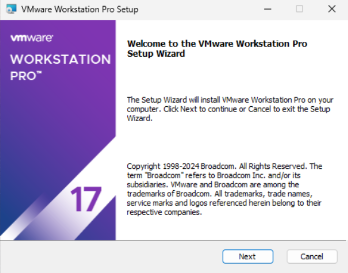
\includegraphics[width=0.8\textwidth]{vmware.png}
		\end{center}
		
	\end{frame}
	
		\begin{frame}
		\frametitle{vmware}
		
		\begin{center}
			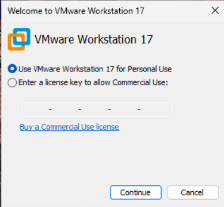
\includegraphics[width=0.6\textwidth]{licensavmware.png}
		\end{center}
		
	\end{frame}
	
	%------------------------------------------------
	
	\begin{frame}
		\frametitle{Cos'è VMware Workstation}
		
		\textbf{VMware Workstation} è un software di virtualizzazione che consente di:
		\begin{itemize}
			\item Creare macchine virtuali (VM)
			\item Eseguire più sistemi operativi su un unico host
			\item Isolare ambienti di test
		\end{itemize}
		
		Vantaggi:
		\begin{itemize}
			\item Sicurezza (isolamento)
			\item Flessibilità
			\item Nessuna modifica al sistema host
		\end{itemize}
		
	\end{frame}
	
	%------------------------------------------------
	
	\begin{frame}
		\frametitle{Download di Debian}
		
		Scaricare Debian dal sito ufficiale:
		
		\begin{itemize}
			\item https://www.debian.org
			\item Sezione: Download
			\item Scegliere versione \textbf{stable}
		\end{itemize}
		
		Tipologie ISO:
		\begin{itemize}
			\item Netinst (consigliata)
			\item DVD completo
		\end{itemize}
		
	\end{frame}
	
	%------------------------------------------------
	
	\begin{frame}
		\frametitle{Creazione della macchina virtuale}
		
		Aprire VMware Workstation:
		
		\begin{itemize}
			\item Click su \textbf{Create a New Virtual Machine}
			\item Selezionare \textbf{Typical (recommended)}
		\end{itemize}
		
		Successivamente:
		\begin{itemize}
			\item Selezionare \textbf{Installer disc image file (ISO)}
			\item Caricare il file ISO di Debian
		\end{itemize}
		
	\end{frame}
	
	
		\begin{frame}
		\frametitle{vmware}
		
		\begin{center}
			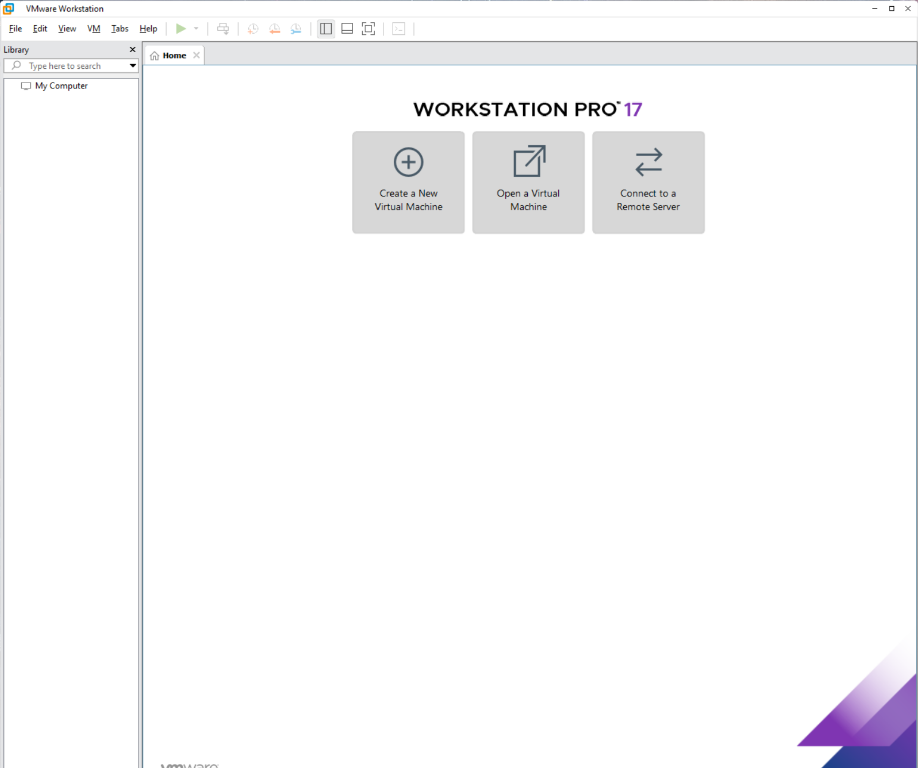
\includegraphics[width=0.9\textwidth]{newvirtualmachine.png}
		\end{center}
		
	\end{frame}
	
	
		\begin{frame}
		\frametitle{vmware}
		
		\begin{center}
			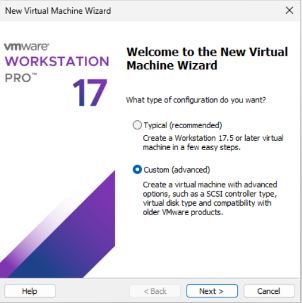
\includegraphics[width=0.6\textwidth]{customvm.png}
		\end{center}
		
	\end{frame}
	
		\begin{frame}
		\frametitle{vmware}
		
		\begin{center}
			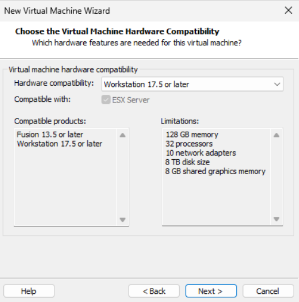
\includegraphics[width=0.6\textwidth]{hardwarecompatibility.png}
		\end{center}
		
	\end{frame}
	
	
	\begin{frame}

Workstation 17.5 or later

Significa che:

La VM utilizzerà le funzionalità più recenti disponibili Sarà compatibile con:

VMware Workstation 17.5+

VMware Fusion 13.5+

Conseguenza importante:

Non potrai aprire facilmente questa VM con versioni più vecchie di VMware

3. Sezione “Compatible products”

Mostra dove potrà essere eseguita la VM:

VMware Fusion 13.5+

VMware Workstation 17.5+

È utile se devi:

spostare la VM tra più ambienti

condividere con altri utenti
	\end{frame}
	%------------------------------------------------
	
		\begin{frame}
		\frametitle{Scaricare ISO Ubuntu}
		
		\begin{center}
			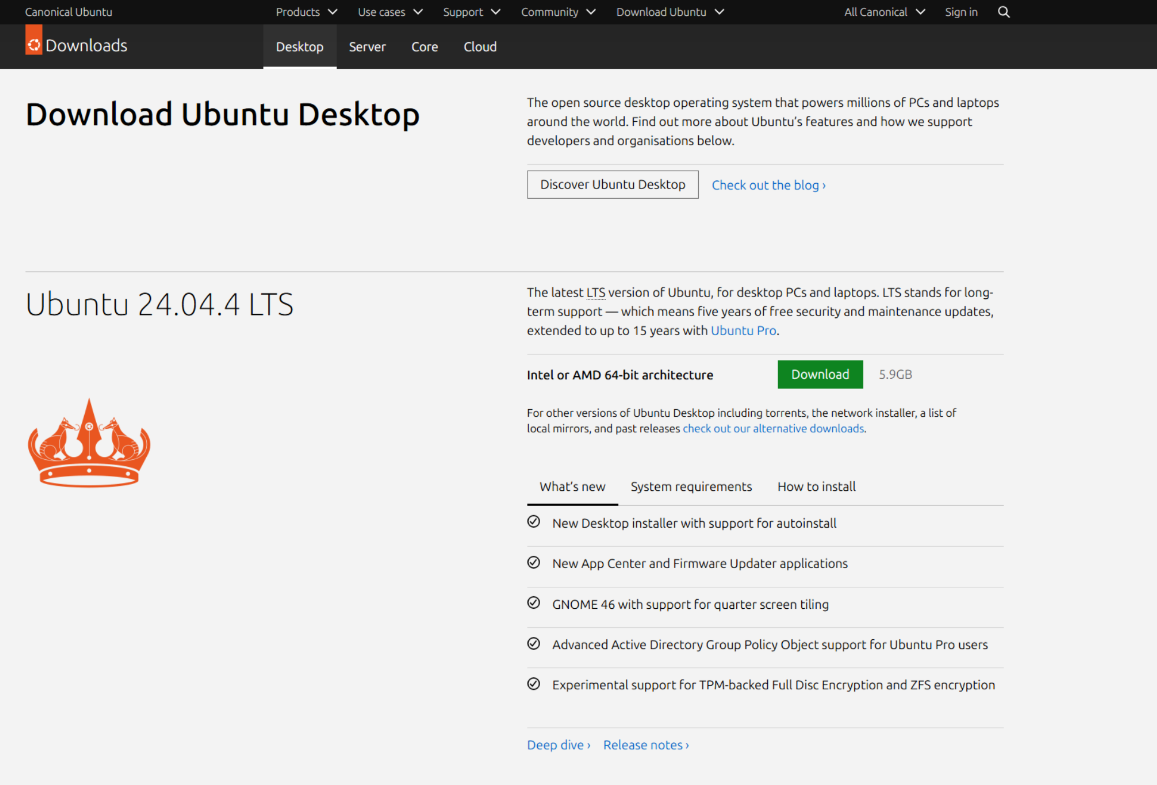
\includegraphics[width=0.8\textwidth]{ubuntu.png}
		\end{center}
		
	\end{frame}
	
		\begin{frame}
		\frametitle{Scaricare ISO Ubuntu}
		
		\begin{center}
			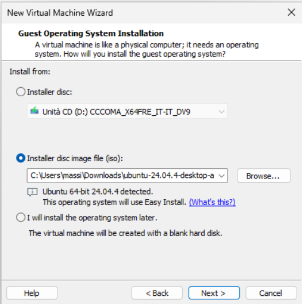
\includegraphics[width=0.6\textwidth]{ubuntu_2.png}
		\end{center}
		
	\end{frame}
	
	\begin{frame}
		\frametitle{Configurazione del sistema operativo}
		
		VMware riconosce automaticamente Ubuntu.
		
		Se non lo fa:
		\begin{itemize}
			\item Selezionare manualmente:
			\begin{itemize}
				\item Linux
				\item Ubuntu (versione corretta)
			\end{itemize}
		\end{itemize}
		
		Assegnare un nome alla VM e scegliere il percorso di salvataggio.
		
	\end{frame}
	
	%------------------------------------------------
	
			\begin{frame}
		\frametitle{Configurazione ISO Ubuntu}
		
		\begin{center}
			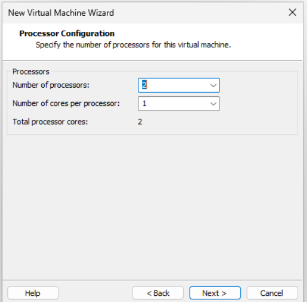
\includegraphics[width=0.6\textwidth]{configurazione_1.png}
		\end{center}
		
	\end{frame}
	
	
	\begin{frame}
		\frametitle{Configurazione hardware}
		
		Impostare le risorse:
		
		\begin{itemize}
			\item RAM: almeno 2 GB (consigliati 4 GB)
			\item CPU: 2 core
			\item Disco: minimo 20 GB
		\end{itemize}
		
		Tipo di disco:
		\begin{itemize}
			\item Consigliato: \textbf{Split into multiple files}
		\end{itemize}
		
	\end{frame}
	
	
		
	\begin{frame}
		\frametitle{Network type}
		
		\begin{center}
			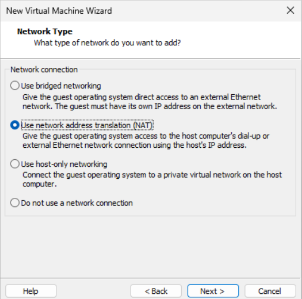
\includegraphics[width=0.6\textwidth]{networktype.png}
		\end{center}
		
	\end{frame}
	
	\begin{frame}
		\frametitle{Tipologie di rete in VMware}
		
		Durante la creazione di una macchina virtuale è possibile scegliere 
		come essa si connette alla rete.
		
		\vspace{0.5cm}
		
		Le principali opzioni sono:
		
		\begin{itemize}
			\item Bridged networking
			\item NAT (Network Address Translation)
			\item Host-only networking
			\item Nessuna connessione di rete
		\end{itemize}
		
		\vspace{0.5cm}
		
		La scelta dipende dal livello di isolamento e accessibilità richiesto.
	\end{frame}
	
	%---------------------------------
	
	\begin{frame}
		\frametitle{Bridged Networking}
		
		\textbf{Caratteristiche}
		\begin{itemize}
			\item La VM è vista come un dispositivo reale nella LAN
			\item Ottiene un indirizzo IP dal router (DHCP)
		\end{itemize}
		
		\vspace{0.4cm}
		
		\textbf{Quando usarlo}
		\begin{itemize}
			\item Server accessibili dalla rete
			\item Test realistici di rete
		\end{itemize}
		
		\vspace{0.4cm}
		
		\textbf{Pro e contro}
		\begin{itemize}
			\item + Massima integrazione
			\item -- Maggiore esposizione
		\end{itemize}
		
	\end{frame}
	
	%---------------------------------
	
	\begin{frame}
		\frametitle{NAT (Network Address Translation)}
		
		\textbf{Caratteristiche}
		\begin{itemize}
			\item La VM usa la connessione dell'host
			\item IP privato non visibile nella LAN
		\end{itemize}
		
		\vspace{0.4cm}
		
		\textbf{Quando usarlo}
		\begin{itemize}
			\item Accesso a Internet semplice
			\item Ambienti di studio e sviluppo
		\end{itemize}
		
		\vspace{0.4cm}
		
		\textbf{Pro e contro}
		\begin{itemize}
			\item + Configurazione automatica
			\item -- Accesso esterno limitato
		\end{itemize}
		
	\end{frame}
	
	%---------------------------------
	
	\begin{frame}
		\frametitle{Host-only e Nessuna rete}
		
		\textbf{Host-only}
		\begin{itemize}
			\item Comunicazione solo con host e altre VM
			\item Nessun accesso a Internet
			\item Ideale per laboratori isolati
		\end{itemize}
		
		\vspace{0.5cm}
		
		\textbf{Nessuna connessione}
		\begin{itemize}
			\item VM completamente isolata
			\item Utile per test offline
		\end{itemize}
		
		\vspace{0.5cm}
		
		\textbf{Sintesi}
		\begin{itemize}
			\item NAT → uso generale
			\item Bridged → visibilità in rete
			\item Host-only → isolamento controllato
		\end{itemize}
		
	\end{frame}
	%------------------------------------------------
	
	\begin{frame}
		\frametitle{Controller type}
		
		\begin{center}
			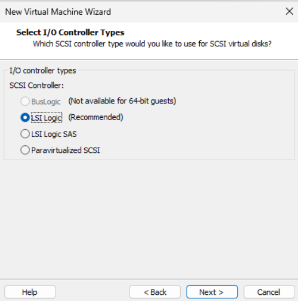
\includegraphics[width=0.6\textwidth]{controllertypes.png}
		\end{center}
		
	\end{frame}
	
	\begin{frame}
		\frametitle{Tipi di Controller SCSI}
		
		Durante la creazione della macchina virtuale, VMware richiede di scegliere
		il tipo di controller per i dischi virtuali.
		
		\vspace{0.5cm}
		
		Le opzioni principali sono:
		
		\begin{itemize}
			\item BusLogic (non disponibile per sistemi a 64 bit)
			\item LSI Logic (consigliato)
			\item LSI Logic SAS
			\item Paravirtualized SCSI (PVSCSI)
		\end{itemize}
		
		\vspace{0.5cm}
		
		La scelta influisce su:
		\begin{itemize}
			\item Compatibilità con il sistema operativo
			\item Prestazioni del disco
			\item Efficienza in ambienti virtualizzati
		\end{itemize}
		
	\end{frame}
	
	%---------------------------------
	
	\begin{frame}
		\frametitle{LSI Logic vs LSI SAS}
		
		\textbf{LSI Logic (consigliato)}
		\begin{itemize}
			\item Massima compatibilità con molti sistemi operativi
			\item Ideale per installazioni standard (es. Debian, Windows)
			\item Non richiede driver aggiuntivi
		\end{itemize}
		
		\vspace{0.4cm}
		
		\textbf{LSI Logic SAS}
		\begin{itemize}
			\item Evoluzione moderna del controller SCSI
			\item Migliori prestazioni rispetto a LSI Logic
			\item Supportato dai sistemi operativi recenti
		\end{itemize}
		
		\vspace{0.4cm}
		
		\textbf{Scelta pratica}
		\begin{itemize}
			\item Uso  generale → LSI Logic
			\item Sistemi moderni o carichi maggiori → LSI SAS
		\end{itemize}
		
	\end{frame}
	
	%---------------------------------
	
	\begin{frame}
		\frametitle{Paravirtualized SCSI (PVSCSI)}
		
		\textbf{Caratteristiche}
		\begin{itemize}
			\item Ottimizzato per ambienti virtualizzati
			\item Prestazioni elevate (I/O intensivo)
		\end{itemize}
		
		\vspace{0.4cm}
		
		\textbf{Attenzione}
		\begin{itemize}
			\item Richiede driver specifici
			\item Potrebbe non essere riconosciuto durante l'installazione del sistema operativo
		\end{itemize}
		
		\vspace{0.4cm}
		
		\textbf{Quando usarlo}
		\begin{itemize}
			\item Server con alto carico disco
			\item Database, applicazioni enterprise
		\end{itemize}
		
		\vspace{0.4cm}
		
		\textbf{Sintesi}
		\begin{itemize}
			\item Semplicità → LSI Logic
			\item Prestazioni avanzate → PVSCSI
		\end{itemize}
		
	\end{frame}
	
		\begin{frame}
		\frametitle{Disk type}
		
		\begin{center}
			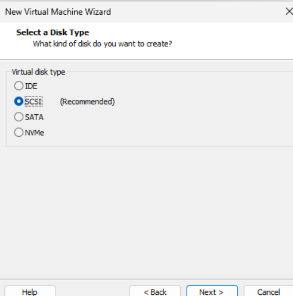
\includegraphics[width=0.6\textwidth]{disktype.png}
		\end{center}
		
	\end{frame}
	
	\begin{frame}
		\frametitle{Tipi di Disco Virtuale}
		
		Durante la creazione della macchina virtuale è necessario scegliere
		il tipo di interfaccia del disco.
		
		\vspace{0.5cm}
		
		Le opzioni disponibili sono:
		
		\begin{itemize}
			\item IDE
			\item SCSI (consigliato)
			\item SATA
			\item NVMe
		\end{itemize}
		
		\vspace{0.5cm}
		
		La scelta influisce su:
		\begin{itemize}
			\item Prestazioni del disco
			\item Compatibilità con il sistema operativo
			\item Efficienza complessiva della VM
		\end{itemize}
		
	\end{frame}
	
	%---------------------------------
	
	\begin{frame}
		\frametitle{IDE e SATA}
		
		\textbf{IDE}
		\begin{itemize}
			\item Tecnologia legacy
			\item Massima compatibilità con sistemi molto vecchi
			\item Prestazioni limitate
		\end{itemize}
		
		\vspace{0.4cm}
		
		\textbf{SATA}
		\begin{itemize}
			\item Più moderno rispetto a IDE
			\item Buon compromesso tra compatibilità e semplicità
			\item Prestazioni medie
		\end{itemize}
		
		\vspace{0.4cm}
		
		\textbf{Quando usarli}
		\begin{itemize}
			\item IDE → sistemi operativi obsoleti
			\item SATA → casi semplici senza esigenze elevate
		\end{itemize}
		
	\end{frame}
	
	%---------------------------------
	
	\begin{frame}
		\frametitle{SCSI (Scelta consigliata)}
		
		\textbf{Caratteristiche}
		\begin{itemize}
			\item Elevate prestazioni rispetto a IDE/SATA
			\item Ottimizzato per ambienti virtualizzati
			\item Supporto diffuso nei sistemi operativi moderni
		\end{itemize}
		
		\vspace{0.4cm}
		
		\textbf{Vantaggi}
		\begin{itemize}
			\item Maggiore efficienza I/O
			\item Migliore gestione di carichi multipli
		\end{itemize}
		
		\vspace{0.4cm}
		
		\textbf{Quando usarlo}
		\begin{itemize}
			\item Uso generale (scelta standard)
			\item Laboratori, sviluppo, server virtuali
		\end{itemize}
		
	\end{frame}
	
	%---------------------------------
	
	\begin{frame}
		\frametitle{NVMe e Sintesi}
		
		\textbf{NVMe}
		\begin{itemize}
			\item Tecnologia moderna ad alte prestazioni
			\item Bassa latenza e alta velocità
			\item Richiede supporto del sistema operativo
		\end{itemize}
		
		\vspace{0.4cm}
		
		\textbf{Quando usarlo}
		\begin{itemize}
			\item Sistemi recenti
			\item Applicazioni ad alto carico I/O
		\end{itemize}
		
		\vspace{0.5cm}
		
		\textbf{Sintesi decisionale}
		\begin{itemize}
			\item Compatibilità → IDE
			\item Semplicità → SATA
			\item Uso generale → SCSI (consigliato)
			\item Prestazioni elevate → NVMe
		\end{itemize}
		
	\end{frame}
	
			\begin{frame}
		\frametitle{Select disk}
		
		\begin{center}
			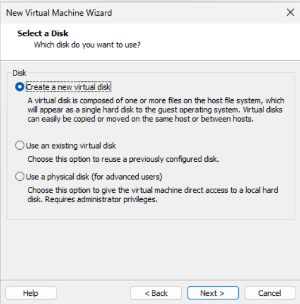
\includegraphics[width=0.6\textwidth]{selectdisk.png}
		\end{center}
		
	\end{frame}
	
	\begin{frame}
		\frametitle{Avvio della macchina virtuale}
		
		Avviare la VM:
		
		\begin{itemize}
			\item Click su \textbf{Power on this virtual machine}
		\end{itemize}
		
		Comparirà il menu di installazione Debian:
		
		\begin{itemize}
			\item Selezionare \textbf{Graphical Install}
		\end{itemize}
		
	\end{frame}
	
	%------------------------------------------------
	
	\begin{frame}
		\frametitle{Installazione Debian - Lingua e localizzazione}
		
		Selezionare:
		\begin{itemize}
			\item Lingua: Italiano
			\item Paese: Italia
			\item Tastiera: Italiana
		\end{itemize}
		
		Queste impostazioni influenzano:
		\begin{itemize}
			\item Locale
			\item Formato data
			\item Layout tastiera
		\end{itemize}
		
	\end{frame}
	
	%------------------------------------------------
	
	\begin{frame}
		\frametitle{Configurazione rete}
		
		Opzioni:
		\begin{itemize}
			\item DHCP (automatico)
			\item Manuale (IP statico)
		\end{itemize}
		
		Per ambienti didattici:
		\begin{itemize}
			\item Usare DHCP
		\end{itemize}
		
		Inserire:
		\begin{itemize}
			\item Nome host
			\item Nome dominio (facoltativo)
		\end{itemize}
		
	\end{frame}
	
	%------------------------------------------------
	
	\begin{frame}
		\frametitle{Utenti e password}
		
		Configurare:
		
		\begin{itemize}
			\item Password root
			\item Utente normale
		\end{itemize}
		
		Buone pratiche:
		\begin{itemize}
			\item Password robuste
			\item Uso di utente non root per attività quotidiane
		\end{itemize}
		
	\end{frame}
	
	%------------------------------------------------
	
	\begin{frame}
		\frametitle{Partizionamento del disco}
		
		Metodo consigliato:
		
		\begin{itemize}
			\item Guidato - usa l'intero disco
		\end{itemize}
		
		Schema:
		\begin{itemize}
			\item Tutti i file in una partizione
		\end{itemize}
		
		Alternativa:
		\begin{itemize}
			\item Partizionamento manuale (avanzato)
		\end{itemize}
		
	\end{frame}
	
	%------------------------------------------------
	
	\begin{frame}
		\frametitle{Installazione del sistema base}
		
		Il sistema installerà:
		\begin{itemize}
			\item Kernel Linux
			\item Pacchetti base
		\end{itemize}
		
		Tempo variabile:
		\begin{itemize}
			\item Dipende da CPU e disco
		\end{itemize}
		
	\end{frame}
	
	%------------------------------------------------
	
	\begin{frame}
		\frametitle{Selezione software}
		
		Scegliere:
		\begin{itemize}
			\item Desktop Environment (GNOME consigliato)
			\item SSH server (opzionale)
			\item Standard system utilities
		\end{itemize}
		
	\end{frame}
	
	%------------------------------------------------
	
	\begin{frame}
		\frametitle{Installazione GRUB}
		
		GRUB è il bootloader.
		
		\begin{itemize}
			\item Installare su disco principale (es. /dev/sda)
		\end{itemize}
		
		Necessario per:
		\begin{itemize}
			\item Avvio del sistema operativo
		\end{itemize}
		
	\end{frame}
	
	%------------------------------------------------
	
	\begin{frame}
		\frametitle{Riavvio e primo accesso}
		
		Al termine:
		\begin{itemize}
			\item Riavviare la macchina virtuale
		\end{itemize}
		
		Accesso:
		\begin{itemize}
			\item Inserire username e password
		\end{itemize}
		
		Verifica:
		\begin{itemize}
			\item Sistema funzionante
			\item Interfaccia grafica attiva
		\end{itemize}
		
	\end{frame}
	
	%------------------------------------------------
	
	\begin{frame}
		\frametitle{Installazione VMware Tools}
		
		Migliora:
		\begin{itemize}
			\item Prestazioni
			\item Grafica
			\item Integrazione mouse
		\end{itemize}
		
		Procedura:
		\begin{itemize}
			\item VM → Install VMware Tools
			\item Montare il CD virtuale
			\item Eseguire script di installazione
		\end{itemize}
		
	\end{frame}
	
	%------------------------------------------------
	
	\begin{frame}
		\frametitle{Conclusioni}
		
		Hai imparato a:
		\begin{itemize}
			\item Creare una macchina virtuale
			\item Installare Debian
			\item Configurare sistema e utenti
		\end{itemize}
		
		Possibili estensioni:
		\begin{itemize}
			\item Snapshot
			\item Networking avanzato
			\item Server Linux
		\end{itemize}
		
	\end{frame}
	
	%------------------------------------------------
	
\end{document}